\documentclass{bioinfo}


\copyrightyear{2019} \pubyear{2019}

\access{Hot Topics in Computational Biology}
\appnotes{Tsinghua University}

\usepackage{algorithm, algorithmic}
\usepackage[utf8]{inputenc}
\usepackage[english]{babel}
\usepackage{amsthm, amsmath, graphicx}
\newtheorem{theorem}{Theorem}
\newtheorem{lemma}{Lemma}

\begin{document}
\firstpage{1}


\subtitle{Gene expression}

\title[SCNet]{SCNet: Unsupervised Multi-Channel Genome Network Inference from Single-Cell RNA Sequences}

%\author[Wang \textit{et~al}.]{Shiyin Wang\,$^{\text{\sfb 1,}*}$}
\author[Wang]{Shiyin Wang\,$^{\text{\sfb 1,}*}$}

\address{$^{\text{\sf 1}}$Institute for Interdisciplinary Information Sciences, Tsinghua University, Beijing, 100084, China}

\corresp{$^\ast$To whom correspondence should be addressed.}

% \history{Received on XXXXX; revised on XXXXX; accepted on XXXXX}

% \editor{Associate Editor: XXXXXXX}

\abstract{\textbf{Motivation:}The rapid advancement of single-cell technologies has shed new light on the complex mechanisms of cellular heterogeneity, as the previous protein networks were ambiguously constructed. Taking advantage of the single-cell expression information can contribute to building reliable next-generation signaling protein networks and conducting causality inference.\\
\textbf{Results:} We proposed an unsupervised causality inference algorithm to extract explainable genome networks from single-cell RNA sequencing results.\\
\textbf{Availability:}The implementation of algorithm SCNet, including source codes and tutorial, is accessible at \url{https://github.com/shiyinw/singlecell\_casuality} with the final version.\\
\textbf{Contact:} \url{wangshiy16@mails.tsinghua.edu.cn}\\
\textbf{Supplementary information:} Supplementary data have been uploaded along with the final version to the Github repo.}

\maketitle




\section{Introduction}


Understanding heterogeneous diseases like cancer on the molecular level are crucial to quantifying the relevant genes and applying precise therapies accordingly.

With the rapid development of computing and biology, advances in sequencing technology have enabled us to profile the RNA sequence in the single-cell level when analyzing genomics, transcriptomics, proteomics, and metabolomics. The rapid advancement of single-cell technologies has shed new light on the complex mechanisms of cellular heterogeneity. Individual single-cell RNA sequencing (scRNA-seq) experiments have already been performed to discover new cell states and reconstruct cellular differentiation trajectories.

The adequacy of experimental data provides opportunities to extract knowledge for the functional relations of genomic entities. The existing protein interaction networks have been widely used in both industry and academia. However, most of the relations are defined in an ambiguous way. Text mining plays a vital role in defining the weights of edges for the sufficiency of text resources. Consequently, we propose employing {\bf{Single-Cell Network (SCNet)}} to utilize single-cell expression profiles for inferring the topology of the protein interaction networks.

Numerous methods have been developed to automatically generate causal directed acyclic graphs (DAGs) upon samples. In reference to those existing techniques, we model single-cell sequences as the samples of the set of transcript genes. We define a probabilistic network model to quantify the likelihood of single-cell sequences on networks. Based on this model, we can then regard it as an optimization problem and solve it accordingly.

We conduct several experiments to test the functionality of SCNet. The result of SCNet is dependent on the provided single-cell sequences. SCNet statistically captures the temporary protein association based on the single-cell expression data. We observe the variation of networks on distinct cell types and find that the dynamic transition of networks aligns with previous experimental traits.


\section{Methods}

\subsection{Probabilistic network model}\label{section:model}

We model the experimental data with a hierarchical Bayesian model. For each pair of variables among genes, the relationship of their expression profiles can show their relationship. We have analyzed the distribution of gene profiles in Figure\ref{figure:dist}. From the data's perspective, we apply the log scale to model the gene expression data in Equation~\ref{equation:model}. Because of the existence of 0 expressed genes, we consider $log(X+1)$ in this equation.


\begin{figure*}
\centering
  
\includegraphics[width=\textwidth]{figure/dist.png}
  \caption{The count plots for the datasets we used in this project. The x-axis is on the log scale. As we can see, we should use a log scale to consider the gene expression level.}
    \label{figure:dist}
\end{figure*}


\begin{equation}
    \begin{array}{ll}
            log(X_i+1) = k_{ij} log(X_j+1) +b\\
            k_{ij} \sim N(\theta_{ij}, \sigma_{ij}^2)\\
    \end{array}
    \label{equation:model}
\end{equation}

Equation~\ref{equation:model} models the pairwise joint distribution of gene expression records. We interpret $k$ as the relation between $X$ and $Y$, and it corresponds to the edge weight in the network.  Therefore, we can get a likelihood representation $Pr(experi|network)$ given the network and gene expression records by calculating the likelihood of $k$.

\begin{equation}
    Pr(net|experi) \propto Pr(experi|net) Pr(net)
    \label{equation:bayesian}
\end{equation}


In Equation~\ref{equation:net}, we assume the prior distribution is Poisson depending on the number of edges in the network. The reason why choose Poisson is because of its nice property of derivative, as shown in Figure~\ref{figure:whypoisson}.

\begin{equation}
    Pr(net) \sim Possion(\lambda)
    \label{equation:net}
\end{equation}

\begin{figure}[H]
\centering
  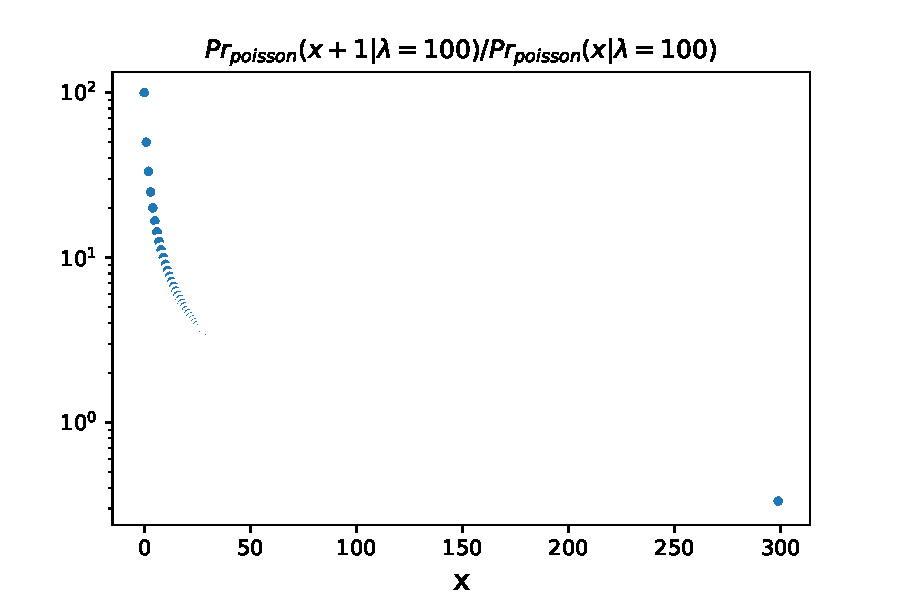
\includegraphics[width=\columnwidth]{figure/whypoisson.pdf}
  \caption{This fraction changes rapidly when $x$ is far away from $\lambda$, while not significant when $x$ is close to $\lambda$. This property can make the number of edges converges fast to the $\lambda$. Therefore, by adjusting parameter $\lambda$, we can guide the sparsity of the network.}
    \label{figure:whypoisson}
\end{figure}

Thus, we can use Bayesian Rule Equation~\ref{equation:bayesian} to get the posterior distribution of the network. And we call the optimized network as {\bf{Single-Cell Network (SCNet)}}. This method can automatically capture the latent relations beneath single-cell gene expression profiles. Moreover, the introduction of prior distribution can flexibly penalize the connection rate of the network.


\subsection{Relaxation on the variance estimation}

If we want to strictly calculate the probability $Pr(experi|net)$, we should estimate both $\theta$ and $\sigma^2$ from the network weights. It is easy to regard the weights as $\theta$, but it is ambiguous to get the variance $\sigma^2$. Alternatively, we assume $\sigma_{experi}^2\approx \sigma_{net}^2$ and acquire the estimation of variance from the gene expression records.

\begin{lemma}[Jackknife Estimate for Variance]
Given n observations $k_0, k_1, \ldots, k_{n-1}$, we want to get the estimate of variance $v$. We can compute the sample median for each subsample omitting the $i$-th observation $\hat{\theta_{i}}=\frac{1}{n-1}(\sum_{j=0}^{n-1} k_j - k_i)$. Then the Jackknife estimate for variance can be acquired by the following function:
\begin{equation}\label{equation:jack}
    v_{jack} = \frac{n-1}{n}\sum_{i=0}^{n-1} (\hat{\theta} - \hat{\theta_{i}})^2
\end{equation}
\end{lemma}


\subsection{Optimization with MCMC}

We use Markov Chain Monte Carlo (MCMC) algorithm to optimize parameters. The transition probability is define as Equation~\ref{equation:accept}. Under the condition that $V(f_1|f_2)$, we can simplify the formula. Finally, we can apply the Equation~\ref{equation:bayesian}.

\begin{equation}\begin{split}
    a(\net_1\rightarrow \net_2)
    & = max\{1, \frac{Pr_{net|experi}(net_2|experi) V(net_1|net_2)}{Pr_{net|experi}(net_1|experi) V(net_2|net_1)}\}\\
    & = max\{1, \frac{Pr_{net|experi}(net_2|experi)}{Pr_{net|experi}(net_1|experi)}\}\\
    & = max\{1, \frac{Pr_{experi|net}(experi|net_2)Pr_{net}(net_2)}{Pr_{experi|net}(experi|net_1)Pr_{net}(net_1)}\}\\
\end{split}\label{equation:bayesian}\end{equation}

\begin{algorithm}[H]
\begin{algorithmic}
\caption{Metropolis-Hastings}
\label{algo:mcmc}
\STATE Compute $log(X+1)$ from gene expression records
\STATE Compute weight means $\theta_{ij}=Pearson(log(X_i+1), log(X_j+1))$
\STATE Compute weight variances $v_{jack}$ by Equation~\ref{equation:jack}
\STATE Initialize network $g^{(0)}$ connections and weights
\FOR{$t$ from $1$ to $N$}
\STATE Randomly choose among actions $\{delete\_an\_edge$, $add\_an\_edge$, $change\_a\_weight\}$ to get a new network $g'$
\STATE Calculate $a=max\{1, \frac{Pr_{y|g}(y|g')Pr_{g}(g')}{Pr_{y|g}(y|g^{(t-1)})Pr_{g}(g^{(t-1)})}\}$
\IF{$random()<= a$}
\STATE Accept this new state $g^{(n)}=g'$ with probability $a$
\ELSE{$g^{(n)}=g^{(n-1)}$}
\ENDIF
\ENDFOR
\end{algorithmic}
\end{algorithm}

\subsection{Datasets and processing}

\begin{figure*}
\centering
  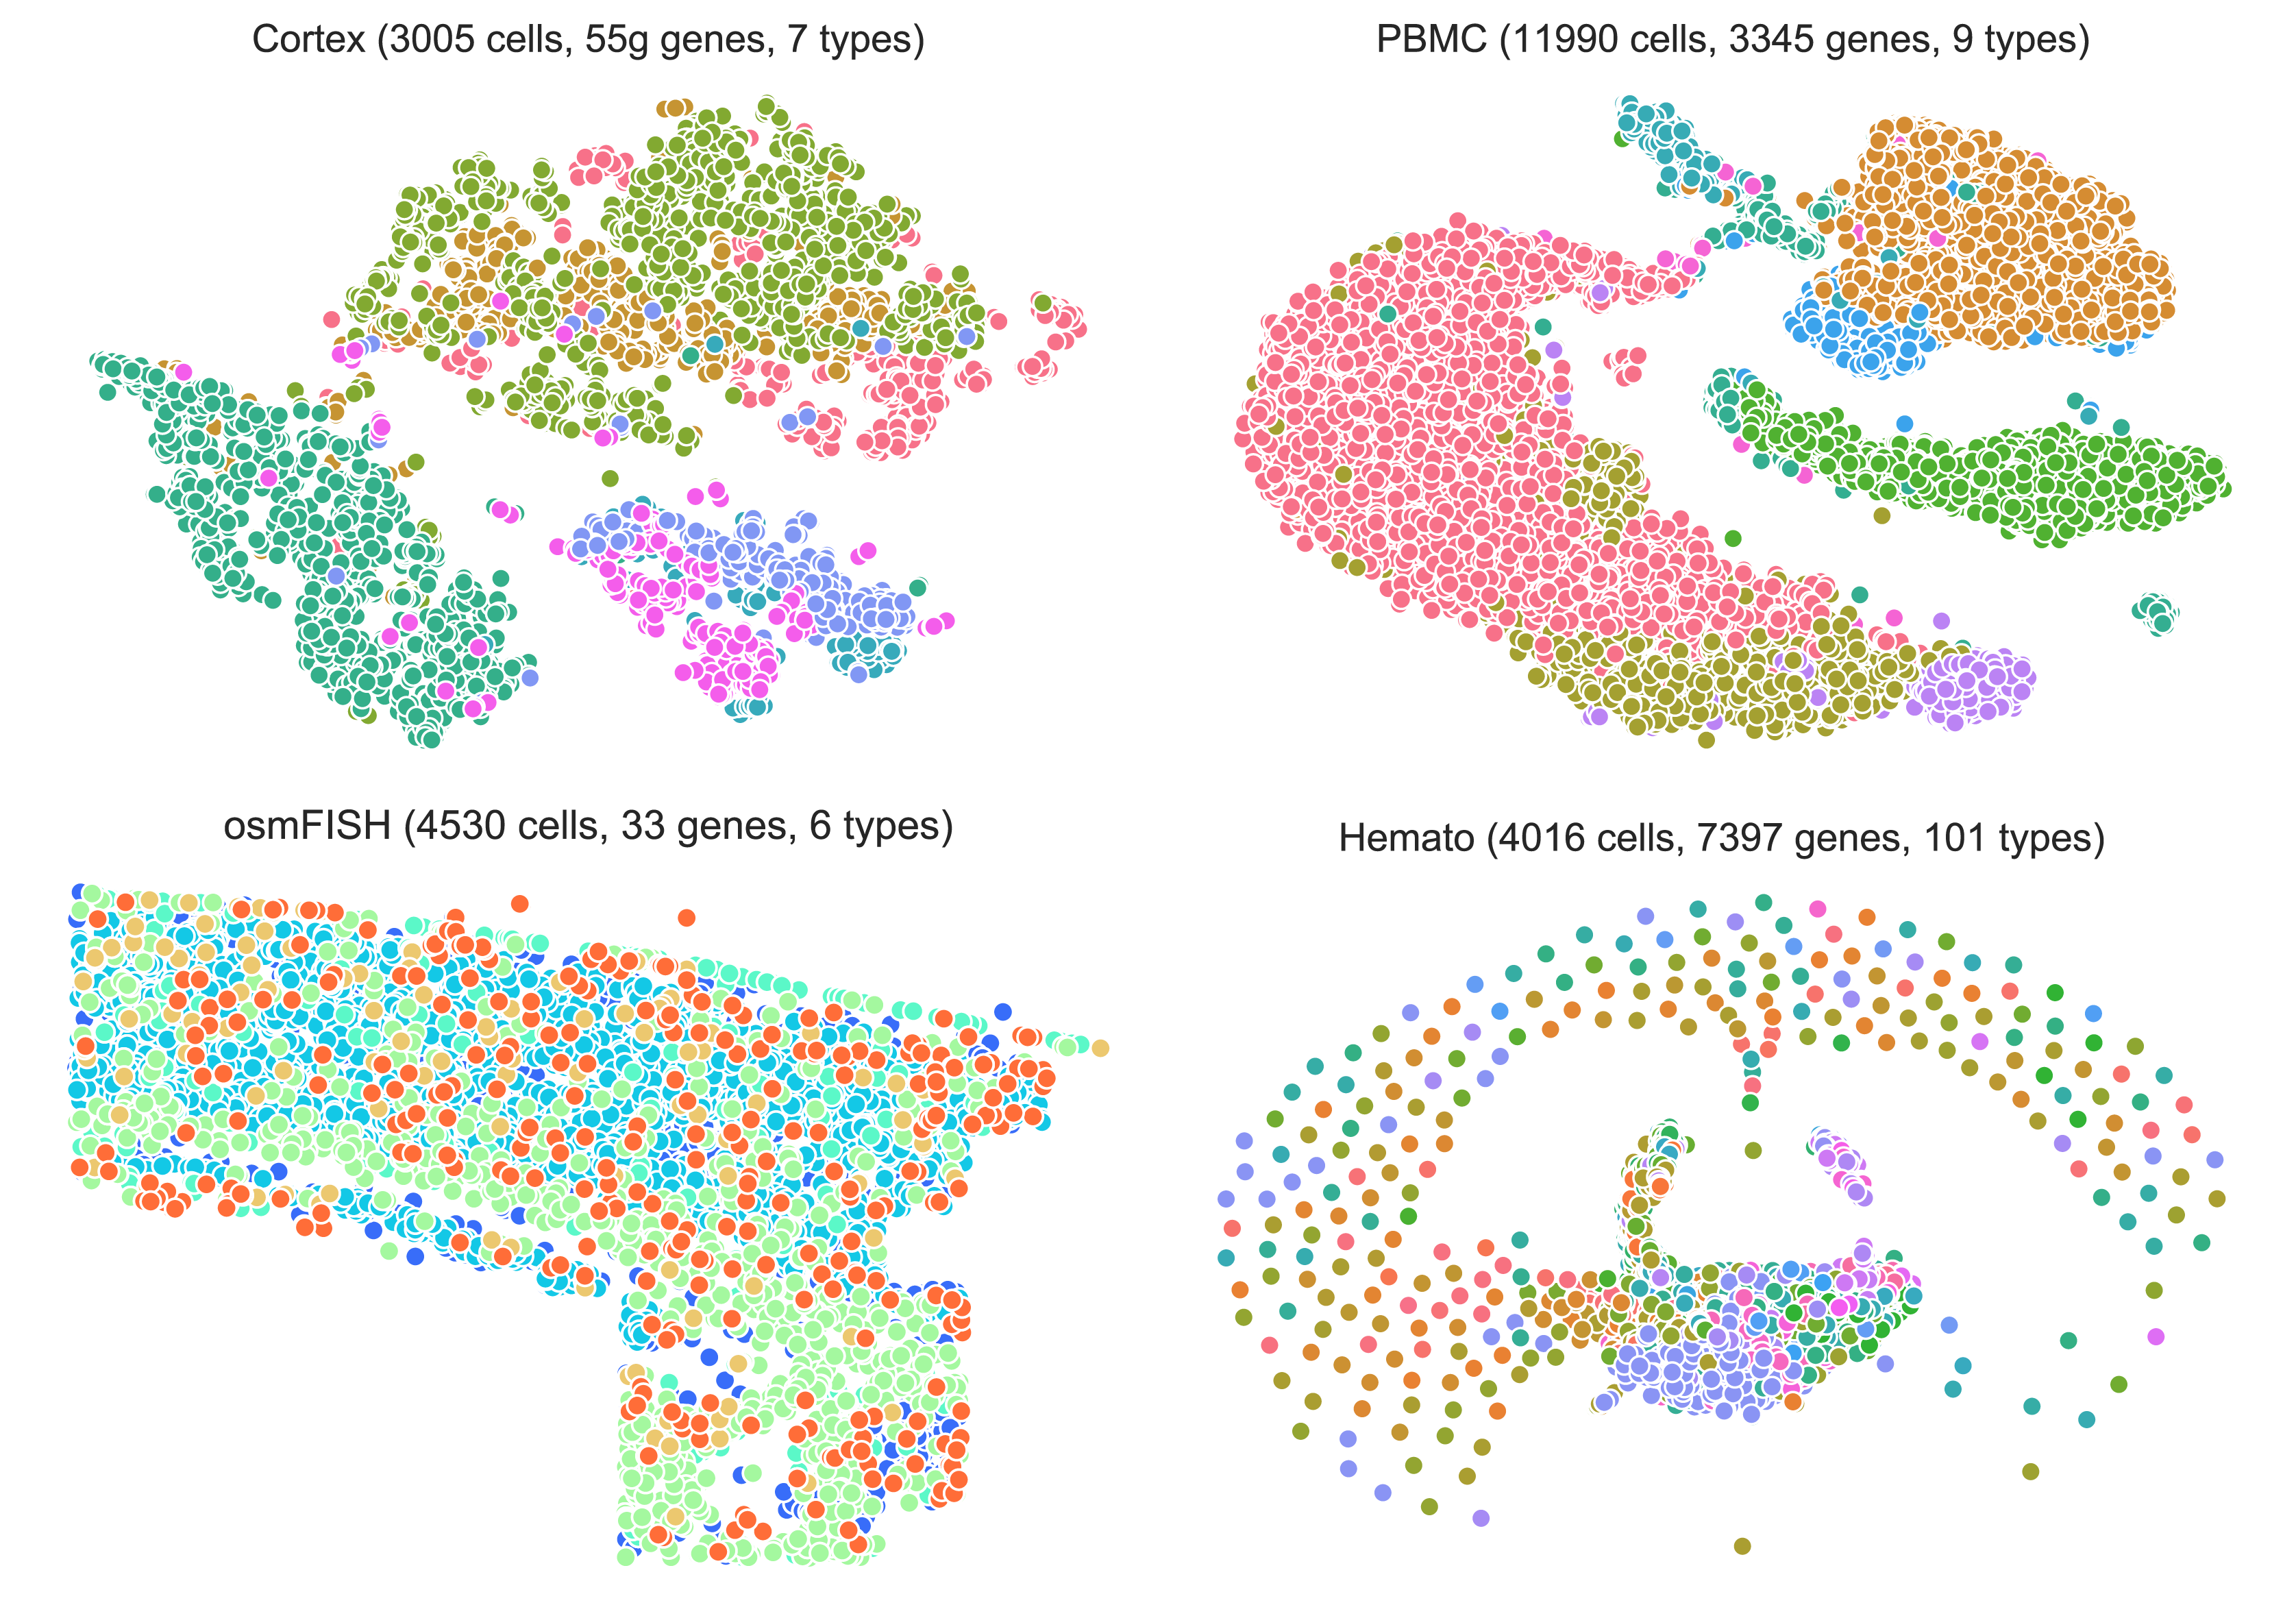
\includegraphics[width=\textwidth]{figure/scatter.png}
  \caption{We use the above four datasets in this project. Except for smFISH which has provided 2-dim positions, all the other datasets are positioned by tSNE results.}\label{scatter}
\end{figure*}


We use multiple annotated datasets in this work. To avoid nasty analysis and amplification, analyze the sequence in the level of genes. We apply the preprocessed data from \citep{gen2018} and used the Python packet scVI \citep{gen2018,scvi2,scvi3,scvi4,scvi5} to process the data. We visualize the datasets in Figure~\ref{scatter}. The osmFISH dataset provides the values of x and y coordinates for each sample. But the other three datasets don't have positions, so we applied tSNE to map the points into 2-dim for visualization.


\paragraph{CORTEX}
The Mouse Cortex Cells dataset from \citep{cortex2015} contains 3,005 mouse cortex cells and gold-standard labels for seven distinct cell types. Each cell type corresponds to a cluster to recover. The researchers in \citep{gen2018} retained the top 558 genes ordered by variance.


\paragraph{Hemato}

The Hemato dataset\cite{hemato} captures continuous gene expression variations. It includes 4,016 cells of 101 gene types from two batches that were profiled using in-drop. This data provides a snapshot of hematopoietic progenitor cells differentiating into various lineages.


\paragraph{PBMC}
Peripheral blood mononuclear cells (PBMCs) dataset from 10x Genomics\citep{x10} consists of 11990 cells on 3346 genes. The work \cite{gen2018} extracted 12,039 cells with 10,310 sampled genes and filtered genes that could not match with the bulk data.

\paragraph{osmFISH}
The research project \cite{smfish} developed a cyclic smFISH protocol, thermed ouroboros smFISH, to quantify the expression of a large number of genes in tissue sections, with the goal to build a cell type map of the mouse somatosensory cortex. We applied the supporting dataset consists of 4530 cells and 33 genes.

\section{Results}
\subsection{Convergence Analysis}
The algorithm converges well, as shown in Figure~\ref{figure:convergence}. Because the network can have multiple variations, it is acceptable that the equilibrium does not stay on a certain network skeleton. Instead, it changes among several network skeletons.

Under appropriate $\lambda$ Poisson prior, the acceptance rate after achieving equilibrium becomes smaller. As discussed in the Figure~\ref{figure:whypoisson}, the $\lambda$ represents the expected number of edges in the network. When the networks are encouraged to have more edges, this method will introduce more noise to the network, and thus changes rapidly under equilibrium.

\begin{figure*}
\centering
  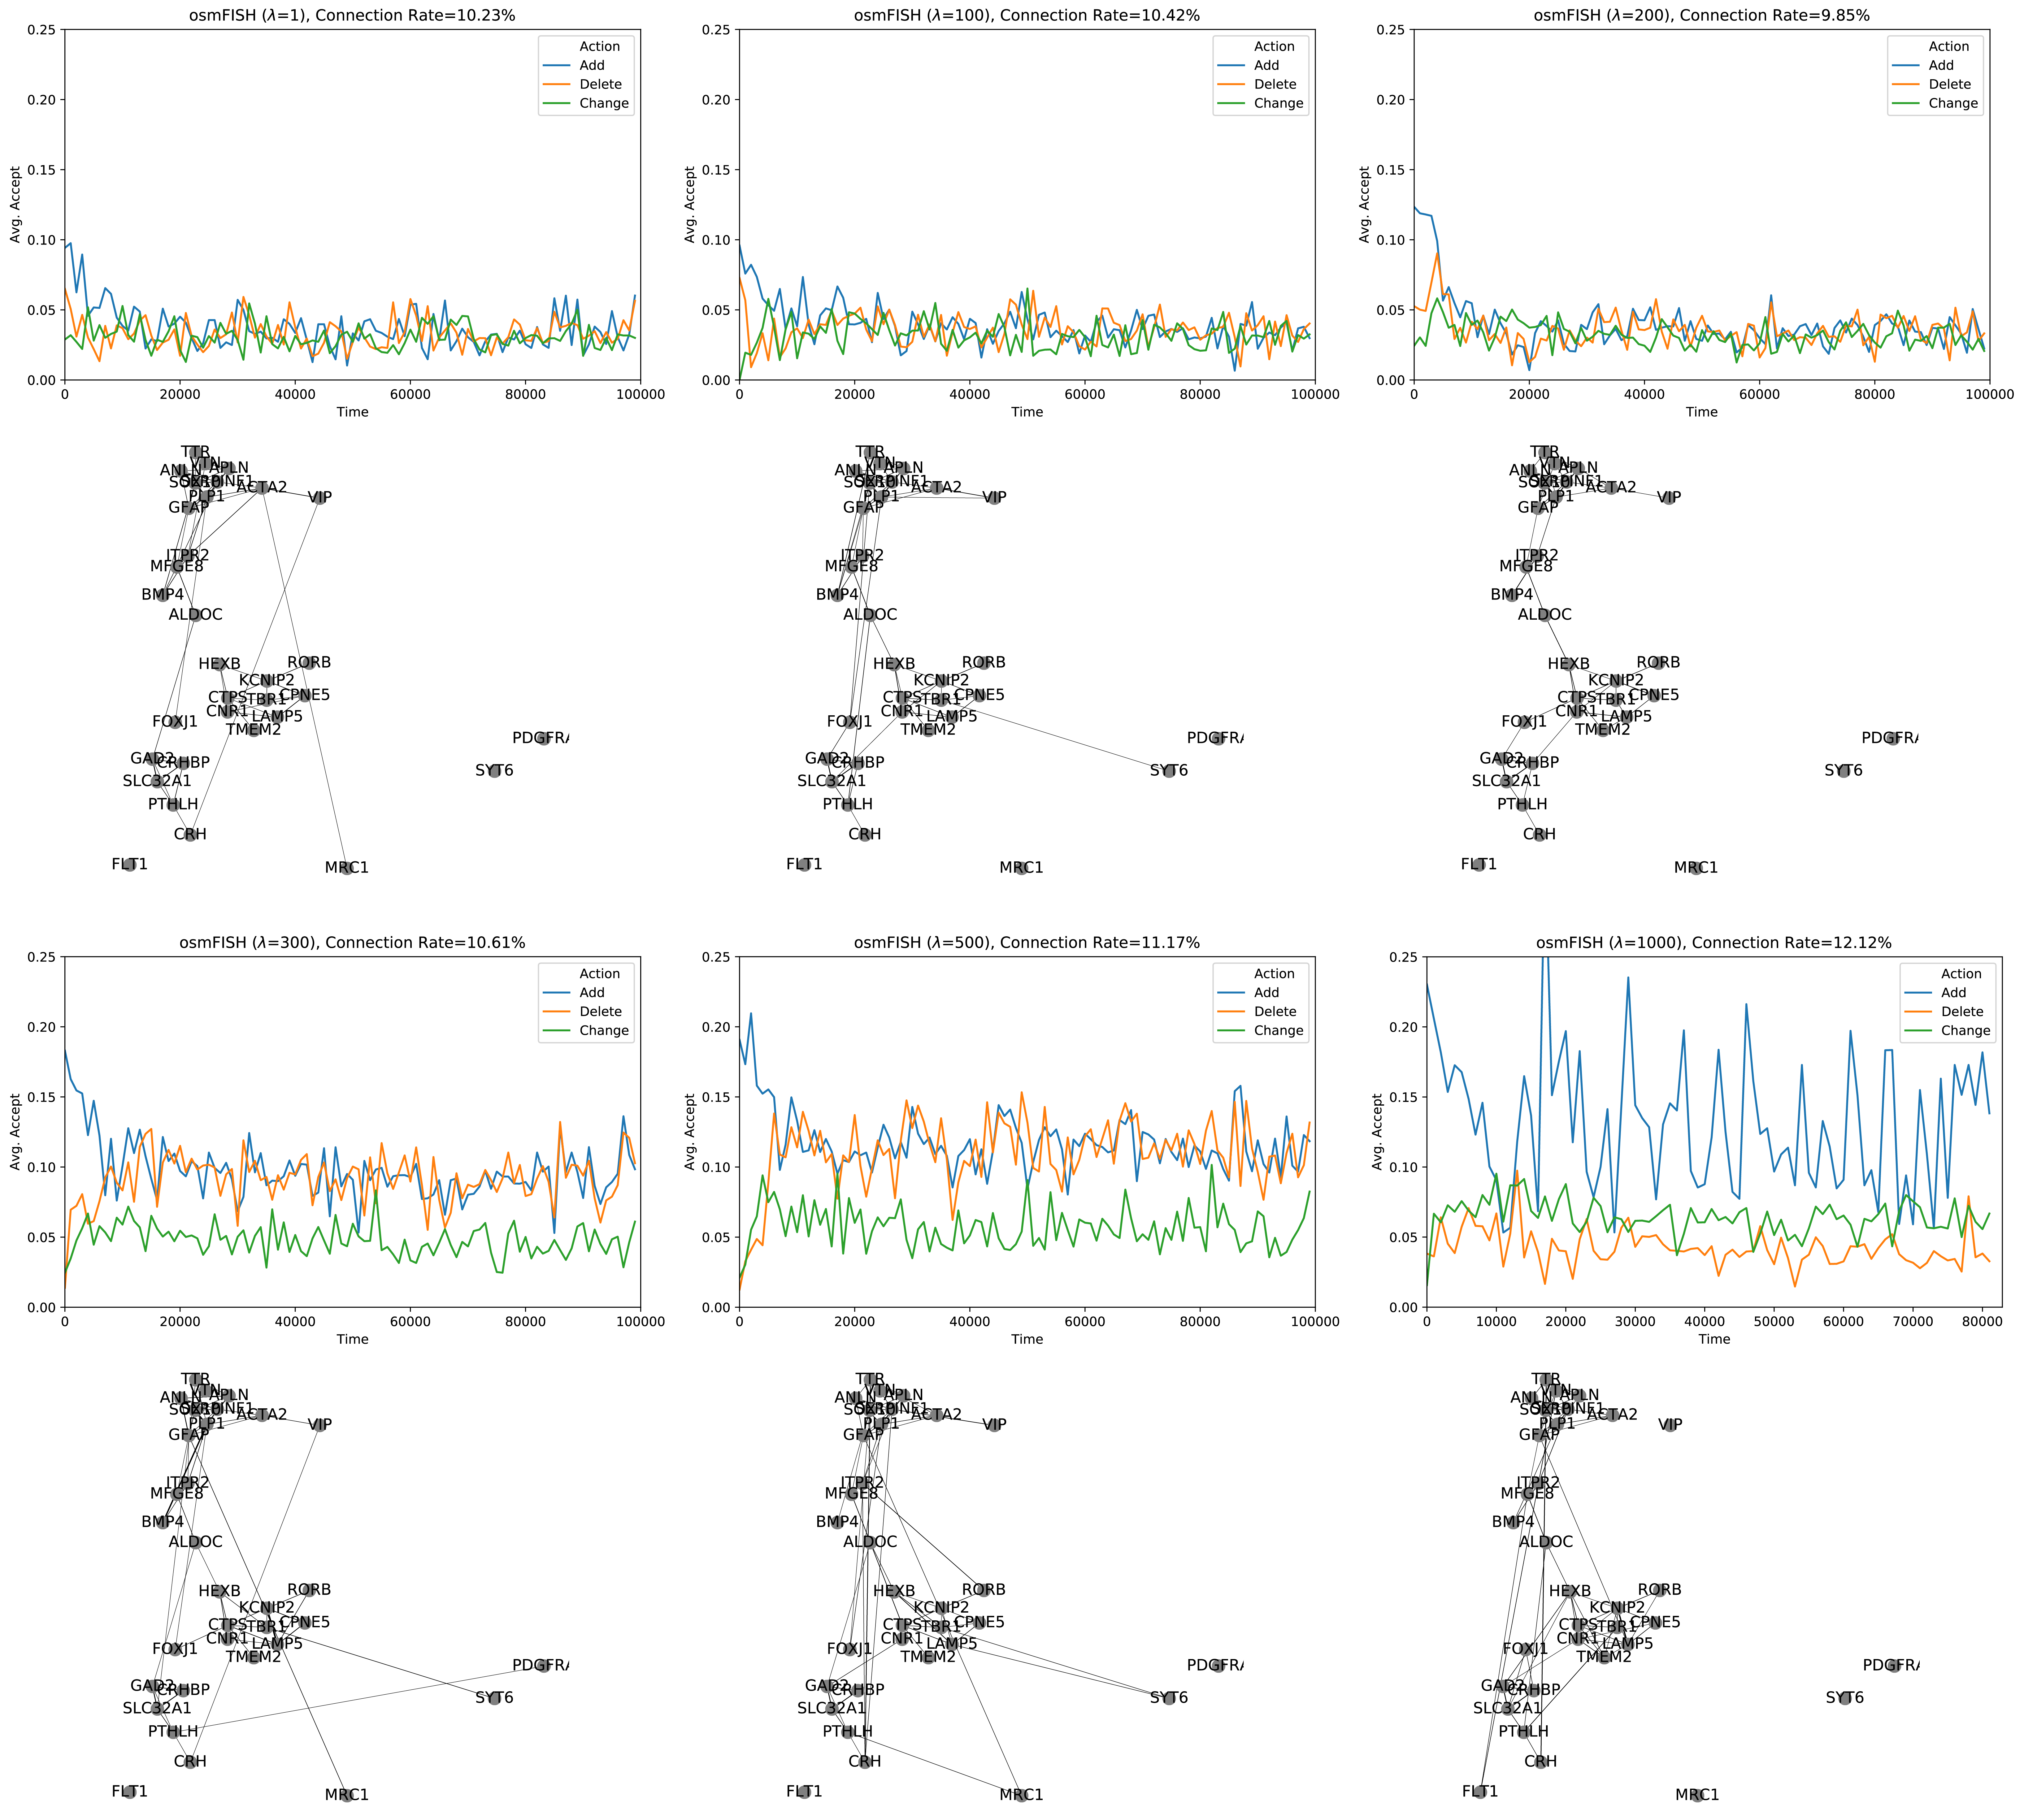
\includegraphics[width=\textwidth]{figure/convergence.png}
  \caption{The average acceptance rate of every 1000 consecutive time steps. "Accept" is recorded as 1 and "Reject" is recorded as 0.}\label{figure:convergence}
\end{figure*}


\subsection{Compare with Gold Standard Provided by Human Experts}
We compare the inferred networks of osmFISH dataset with the existing database STRING to acquire supporting evidence for our method. Figure~\ref{fig:string} is the result provided by the STRING database. Our network has a similar topology with this result. There are ten correctly inferred edges in our SCNet. There are 55 edges in the SCNet and 39 edges in the string network. The true positive is 10. Many difference occurs in the text mining channel. We interpret that our SCNet method should be equipped with expert knowledge, and it also has the potential to capture more hidden information.

\begin{figure}[H]
    \centering
    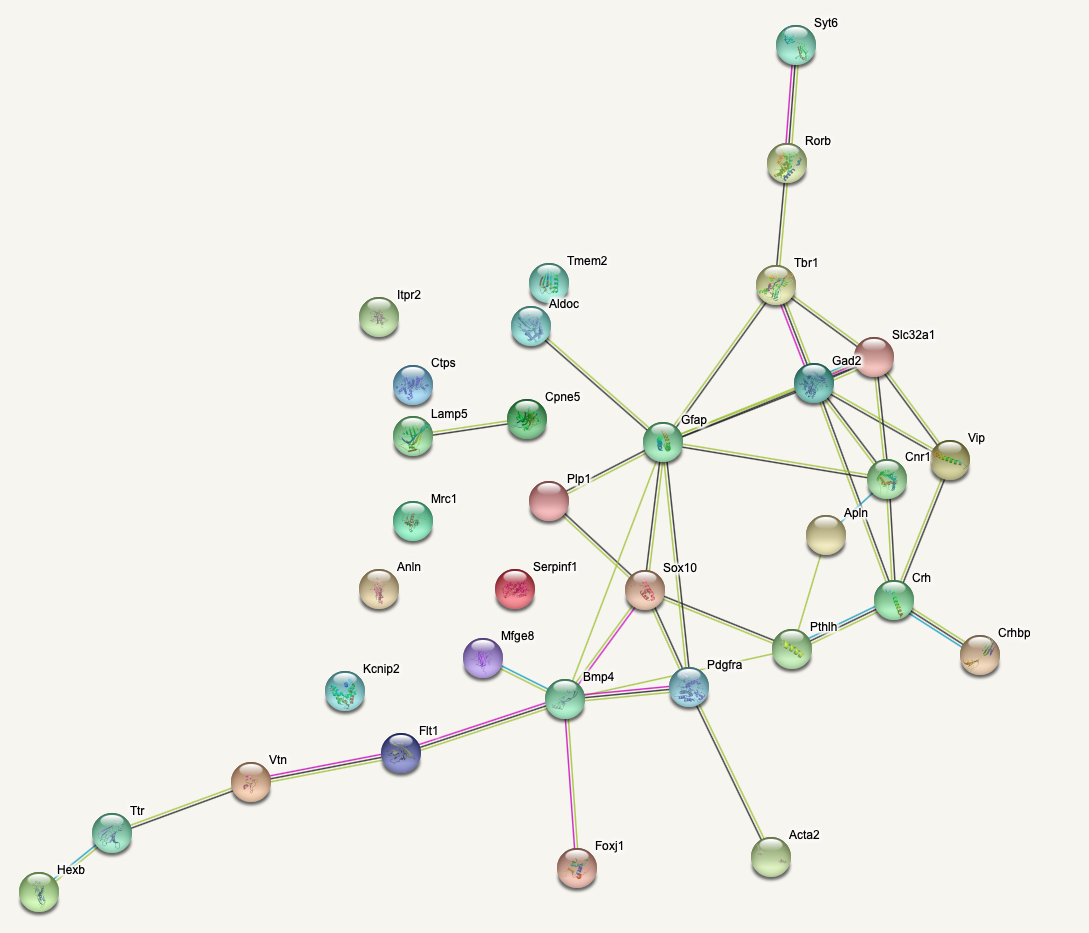
\includegraphics[width=\columnwidth]{figure/string.png}
    \caption{The search result for the 33 genes shown in the osmFISH dataset.}
    \label{fig:string}
\end{figure}

\section{Discussion}

In this paper, we proposed an unsupervised causality inference algorithm to extract explainable genome networks from single-cell RNA sequencing results.

We first statistically build a probabilistic model theoretically bridge the experimental records and network skeleton. To simplify the optimization process, we apply relaxation for the variance estimation. We also discuss the distribution choice of Poisson in our model. We finally apply the MCMC estimation algorithm to calculate the optimum networks.

Then we apply our method to several datasets, especially on osmFISH, which has considerably fewer gene sets. We compare the result of SCNet with STRING database and discuss the performance. Though the performance is not persuasive enough to predict the connections, it provides insights on which edge may have errors.

There are several future directions following our project:

\begin{itemize}
    \item Apply the network to see gene types variations.
    \item Deploy methods to correct existing network databases automatically.
    \item Theoretical analysis to compare with other methods that derive networks from the covariance matrix directly.
\end{itemize}




%%%%%%%%%%%%%%%%%%%%%%%%%%%%%%%%%%%%%%%%%%%%%%%%%%%%%%%%%%%%%%%%%%%%%%%%%%%%%%%%%%%%%
%
%     please remove the " % " symbol from \centerline{\includegraphics{fig01.eps}}
%     as it may ignore the figures.
%
%%%%%%%%%%%%%%%%%%%%%%%%%%%%%%%%%%%%%%%%%%%%%%%%%%%%%%%%%%%%%%%%%%%%%%%%%%%%%%%%%%%%%%

% \input{template.tex}

\section*{Acknowledgements}

This is the final course project of "Hot Topics in Computational Biology" supervised by Professor Jianyang Zeng at Tsinghua University in the 2019 autumn semester.

% \section*{Funding}

% This work is not supported by any funding.

\bibliographystyle{natbib}
\bibliographystyle{achemnat}
\bibliographystyle{plainnat}
\bibliographystyle{abbrv}
\bibliographystyle{bioinformatics}
\bibliographystyle{plain}

\nocite{*}
\bibliography{Document}

\end{document}
